\documentclass[border=10pt]{standalone}
\usepackage{tikz}
\usepackage{amsmath}
\usetikzlibrary{shapes, arrows, calc, positioning}

\begin{document}
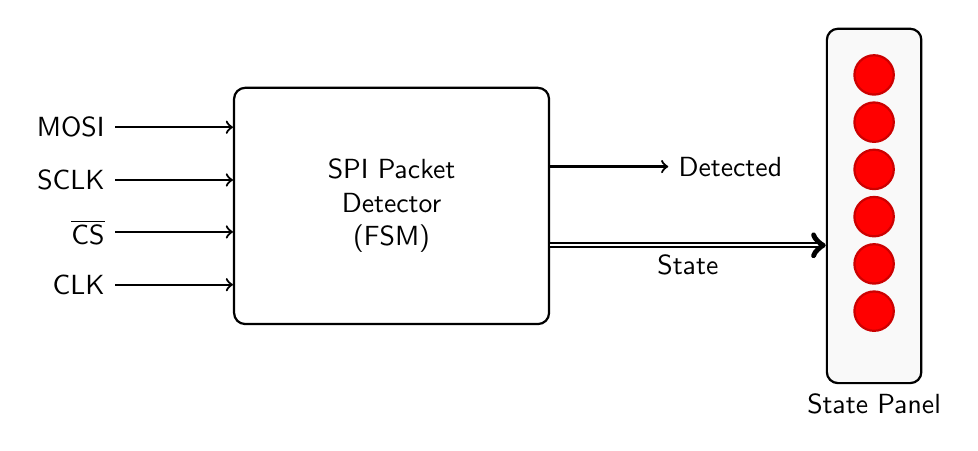
\begin{tikzpicture}[
    font=\sffamily,
    thick,
    box/.style={
        draw, 
        rectangle, 
        minimum width=4cm, 
        minimum height=3cm, 
        rounded corners, 
        fill=white, 
        align=center
    },
    input/.style={
        coordinate
    },
    output/.style={
        coordinate
    },
    led/.style={
        circle,
        draw=red!80!black,
        fill=red,
        inner sep=0pt,
        minimum size=0.5cm
    }
]

    % Main Block
    \node [box] (system) {SPI Packet\\Detector\\(FSM)};

    % Inputs
    \coordinate (mosi) at ($(system.west) + (0, 1)$);
    \coordinate (sclk) at ($(system.west) + (0, 0.33)$);
    \coordinate (cs) at ($(system.west) + (0, -0.33)$);
    \coordinate (clk) at ($(system.west) + (0, -1)$);

    \draw [<-] (mosi) -- ++(-1.5, 0) node [left] {MOSI};
    \draw [<-] (sclk) -- ++(-1.5, 0) node [left] {SCLK};
    \draw [<-] (cs) -- ++(-1.5, 0) node [left] {$\overline{\text{CS}}$};
    \draw [<-] (clk) -- ++(-1.5, 0) node [left] {CLK};

    % Output - Detected
    \coordinate (detected) at ($(system.east) + (0, 0.5)$);
    \draw [->] (detected) -- ++(1.5, 0) node [right] {Detected};

    % State Panel
    \node [draw, rounded corners, rectangle, right=3.5cm of system, minimum width=1.2cm, minimum height=4.5cm, label=below:State Panel, fill=gray!5] (panel) {};
    
    % State Bus Connection
    \draw [->, double] ($(system.east) + (0, -0.5)$) -- ($(panel.west) + (0, -0.5)$) node [midway, below] {State};

    % LEDs in the panel
    \foreach \i [evaluate=\i as \ypos using -0.6-(5-\i)*0.6] in {5,4,...,0} {
        \node [led] at ($(panel.north) + (0, \ypos)$) {};
    }

\end{tikzpicture}
\end{document}
